\documentclass{beamer}

\mode<presentation>
{
  \usetheme{CambridgeUS}
  \setbeamercovered{transparent}
}

\usepackage{color}
\usepackage[ampersand]{easylist}
\usepackage[english]{babel}
\usepackage[latin1]{inputenc}
\usepackage{times}
\usepackage[T1]{fontenc} 
% Or whatever. Note that the encoding and the font should match. If T1
% does not look nice, try deleting the line with the fontenc.
\usepackage{amsmath}

\newcommand{\linespace}{\vskip 0.25cm}

\definecolor{MyForestGreen}{rgb}{0,0.7,0} 
\newcommand{\tableemph}[1]{{#1}}
\newcommand{\tablewin}[1]{\tableemph{#1}}
\newcommand{\tablemid}[1]{\tableemph{#1}}
\newcommand{\tablelose}[1]{\tableemph{#1}}

\definecolor{MyLightGray}{rgb}{0.6,0.6,0.6}
\newcommand{\tabletie}[1]{\color{MyLightGray} {#1}}

% The text in square brackets is the short version of your title and will be used in the
% header/footer depending on your theme.
\title[Applying EC to Robotics]{Applying Evolutionary Computation to Robotics}

% Sub-titles are optional - uncomment and edit the next line if you want one.
% \subtitle{Why does sub-tree crossover work?} 

% The text in square brackets is the short version of your name(s) and will be used in the
% header/footer depending on your theme.
\author[Schiller]{Adrian Thomas Schiller}

% The text in square brackets is the short version of your institution and will be used in the
% header/footer depending on your theme.
\institute[U of Minn, Morris]
{
  Division of Science and Mathematics \\
  University of Minnesota, Morris \\
  Morris, Minnesota, USA
}

% The text in square brackets is the short version of the date if you need that.
\date%[July '09, GECCO, Montr\'{e}al] % (optional)
{28 April 2014}

% Delete this, if you do not want the table of contents to pop up at
% the beginning of each subsection:
\AtBeginSection[]
{
  \begin{frame}<beamer>
    \frametitle{Outline}
    \tableofcontents[currentsection, hideothersubsections]
  \end{frame}
}

\begin{document}

\begin{frame}
  \titlepage
\end{frame}

\section*{Overview}
\subsection*{}
\begin{frame}
  \frametitle{The Big Picture}
  \begin{itemize}
    \item \textbf{Problem}: A robot is faced with a problem where the solution is not immediately obvious
        \item \textbf{Potential Solution}: Evolutionary computation (EC) is a process which can can solve difficult problems in programming
        \item \textbf{Issue}: Since a robot interacts with the physical world, EC is slower by many magnitudes 
        \item \textbf{Solution}: By using simulation and applicable evolutionary strategies, it is possible to use EC to evolve robots
  \end{itemize}

\end{frame}

%\subsection{Intro2}
%\begin{frame}
 % \frametitle{Introduce solving cases}
%\end{frame}

\section{Background}
	\subsection{Evolutionary Computation}
\begin{frame}
\frametitle{Evolutionary Computation}
 \begin{itemize}
\item Evolutionary Computation (EC) is a problem solving technique which mimics natural selection
\item EC requires:
\begin{itemize}
  \item A candidate representation of a potential solution
  \item A population of randomly generated candidates
  \item A fitness function
\end{itemize}
  \end{itemize}
\end{frame}

\begin{frame}
\frametitle{Evolutionary Computation: Process}
 \begin{itemize}
  \item Candidates are evaluated
  \item The best performing candidates are selected
  \item Selected candidates undergo Transformations to repopulate the population
  \item Process repeats until some limit is reached
\end{itemize}
\end{frame}

%\subsection{Genetic Algorithm}
%\begin{frame}
 % \frametitle{Genetic Algorithm}
%\begin{itemize}
 % \item Genetic Algorithms are a type of EC
 % \item Candidates are represented as bit strings
%\end{itemize}
%\end{frame}

%\begin{comment}
%\begin{frame}
%
%  \frametitle{Genetic Algorithm: Cross-over}
%\begin{itemize}
%  \item A Cross-over point is selected from two candidates. All bits are swapped beyond the point, creating two new candidates.
%\end{itemize}
%  \begin{columns}
%  \begin{column}{0.5\textwidth}
%\begin{itemize}
%  \item Before:
%\end{itemize}
%\[
%C_i=[ \textcolor{red}{1},  \textcolor{red}{0}, \textcolor{red}{1},  \textcolor{red}{0},|  \textcolor{red}{0},  \textcolor{red}{0}, %\textcolor{red}{1}, \textcolor{red}{0}, \textcolor{red}{0}, \textcolor{red}{1} ]
%\]
%\[C_j=[  \textcolor{blue}{0}, \textcolor{blue}{0}, \textcolor{blue}{1}, \textcolor{blue}{1},| \textcolor{blue}{0}, \textcolor{blue}{1}, \textcolor{blue}{1}, \textcolor{blue}{0}, \textcolor{blue}{1}, \textcolor{blue}{0} ]
%\]
%\end{column}
% \begin{column}{0.5\textwidth}
%\begin{itemize}
%  \item After:
%\end{itemize}
%   \[
%[ \textcolor{red}{1},  \textcolor{red}{0}, \textcolor{red}{1},  \textcolor{red}{0}, \textcolor{blue}{0}, \textcolor{blue}{1}, %\textcolor{blue}{1}, \textcolor{blue}{0}, \textcolor{blue}{1}, \textcolor{blue}{0} ]
%\]
%\[ [  \textcolor{blue}{0}, \textcolor{blue}{0}, \textcolor{blue}{1}, \textcolor{blue}{1}, \textcolor{red}{0},  \textcolor{red}{0}, %\textcolor{red}{1}, \textcolor{red}{0}, \textcolor{red}{0}, \textcolor{red}{1} ]
%\]
%  \end{column}
%  \end{columns}
%\end{frame}
%
%\begin{frame}
%  \frametitle{Genetic Algorithm: Candidate Manipulation}
%%\begin{itemize}
%  \item Mutation:
%\end{itemize}
%\[
%[ \textcolor{red}{1},  \textcolor{red}{0}, \textcolor{red}{1},  \textcolor{red}{0},  \textcolor{red}{0},  \textcolor{red}{0}, %\textcolor{red}{1}, \textcolor{red}{0}, \textcolor{red}{1}, \textcolor{red}{1} ]
%\]
%\[[ \textcolor{red}{1},  \textcolor{red}{0}, \textcolor{red}{1},  \textcolor{red}{0},  \textcolor{red}{0},  \textcolor{red}{0}, %\textcolor{red}{1}, \textcolor{red}{0}, \textcolor{blue}{0}, \textcolor{red}{1} ]
%\]
%\end{frame}
%\end{comment}


\subsection*{``One Max'' Example}
\begin{frame}
  \frametitle{Example: ``One Max''}
\begin{itemize}
\item Goal: Evolve an array consisting of the most ones from 20 candidate arrays with 10 bits
\end{itemize}
\[
20 \left\{\begin{matrix}
[  1,~1,~1,~0,~ 0,~0,~1,~0,~0,~1] \\ %inkscape, omnigraphle, googledocs? (need pdf vector graphic)
[  0,~0,~1,~1,~ 0,~1,~1,~0,~1,~0] \\
\cdots\\
[  1 ,~0,~1,~0,~ 1,~1,~1,~0,~0,~0] 
\end{matrix}\right.
\]
\end{frame}

\begin{frame}
  \frametitle{Fitness Evaluation}
\begin{itemize}
\item The fitness function $F()$ is used to calculate the fitness of each candidate
\item In this case, the function counts the number of ones in the array
\end{itemize}

\[F([   \textcolor{red}{1},~\textcolor{red}{1},~ \textcolor{red}{1},~0,~ 0,~0,~\textcolor{red}{1},~ 0,~ 0,~ \textcolor{red}{1}]  ) = 6 \]%inkscape, omnigraphle, googledocs? (need pdf vector graphic)
\[F([  0 ,~0,~ \textcolor{red}{1},~ \textcolor{red}{1},~ 0,~ \textcolor{red}{1},~ \textcolor{red}{1},~0,~ \textcolor{red}{1},~0]) = 4\]
\[\cdots\]
\[F([   \textcolor{red}{1},~0,~ \textcolor{red}{1},~0,~  \textcolor{red}{1},~ \textcolor{red}{1},~ \textcolor{red}{1},~0,~0,~0]) = 5\]
\end{frame}

\begin{frame}
  \frametitle{Cross-Over}
\begin{itemize}
\item The top 10 candidates are selected to create a new population
\item Top candidates are randomly selected to cross-over with one another
\end{itemize}

  \begin{columns}
  \begin{column}{0.5\textwidth}

\[
C_1=[ \textcolor{red}{1},  \textcolor{red}{1}, \textcolor{red}{1},  \textcolor{red}{0},|  \textcolor{red}{0},  \textcolor{red}{0}, \textcolor{red}{1}, \textcolor{red}{0}, \textcolor{red}{0}, \textcolor{red}{1} ]
\]
\[C_2=[  \textcolor{blue}{0}, \textcolor{blue}{0}, \textcolor{blue}{1}, \textcolor{blue}{1},| \textcolor{blue}{0}, \textcolor{blue}{1}, \textcolor{blue}{1}, \textcolor{blue}{0}, \textcolor{blue}{1}, \textcolor{blue}{0} ]
\]
\end{column}
 \begin{column}{0.5\textwidth}

   \[
C_x=[ \textcolor{red}{1},  \textcolor{red}{1}, \textcolor{red}{1},  \textcolor{red}{0}, \textcolor{blue}{0}, \textcolor{blue}{1}, \textcolor{blue}{1}, \textcolor{blue}{0}, \textcolor{blue}{1}, \textcolor{blue}{0} ]
\]
\[C_y = [  \textcolor{blue}{0}, \textcolor{blue}{0}, \textcolor{blue}{1}, \textcolor{blue}{1}, \textcolor{red}{0},  \textcolor{red}{0}, \textcolor{red}{1}, \textcolor{red}{0}, \textcolor{red}{0}, \textcolor{red}{1} ]
\]
  \end{column}
  \end{columns}
\end{frame}

\begin{frame}
  \frametitle{Mutation}
\begin{itemize}
  \item Some created candidates may undergo mutation:
\end{itemize}
\[
C_x=[ \textcolor{red}{1},  \textcolor{red}{1}, \textcolor{red}{1},  \textcolor{red}{0}, \textcolor{red}{0}, \textcolor{red}{1}, \textcolor{red}{1}, \textcolor{red}{0}, \textcolor{red}{1}, \textcolor{red}{0} ]
\]
\[C_x'=[ \textcolor{red}{1},  \textcolor{red}{1}, \textcolor{red}{1},  \textcolor{red}{0}, \textcolor{blue}{1}, \textcolor{red}{1}, \textcolor{red}{1}, \textcolor{red}{0}, \textcolor{red}{1}, \textcolor{red}{0} ]
\]
\end{frame}

\begin{frame}
  \frametitle{Repeat}
\begin{itemize}
  \item Once the population is recreated, the process repeats until eventually a limit is reached
  \item In this case, the limit would be iterations, time, or finding an array of all 1's
\end{itemize}
\[
F([ \textcolor{red}{1},  \textcolor{red}{1}, \textcolor{red}{1}, 0, \textcolor{red}{1}, \textcolor{red}{1}, \textcolor{red}{1}, 0, \textcolor{red}{1}, 0 ]) = 7
\]
\[F([  0, 0, \textcolor{red}{1}, \textcolor{red}{1}, 0,  0, \textcolor{red}{1}, 0, 0, \textcolor{red}{1} ]) = 4
\]
\[\cdots\]
\[F([  \textcolor{red}{1}, 0, \textcolor{red}{1}, \textcolor{red}{1}, 0,  \textcolor{red}{1}, 0, 0, \textcolor{red}{1}, \textcolor{red}{1} ]) = 6
\]
\end{frame}

\subsection{Artificial Neural Networks}
\begin{frame}
  \frametitle{Artificial Neural Networks (ANN)}
\begin{columns}
  \begin{column}{0.5\textwidth}
\begin{itemize}
\item  ANNs are a collection of nodes with weighted vertices.
\item The purpose of the network is to develop a functional relationship from the input to the output
\end{itemize}
\end{column}
\begin{column}{0.5\textwidth}
 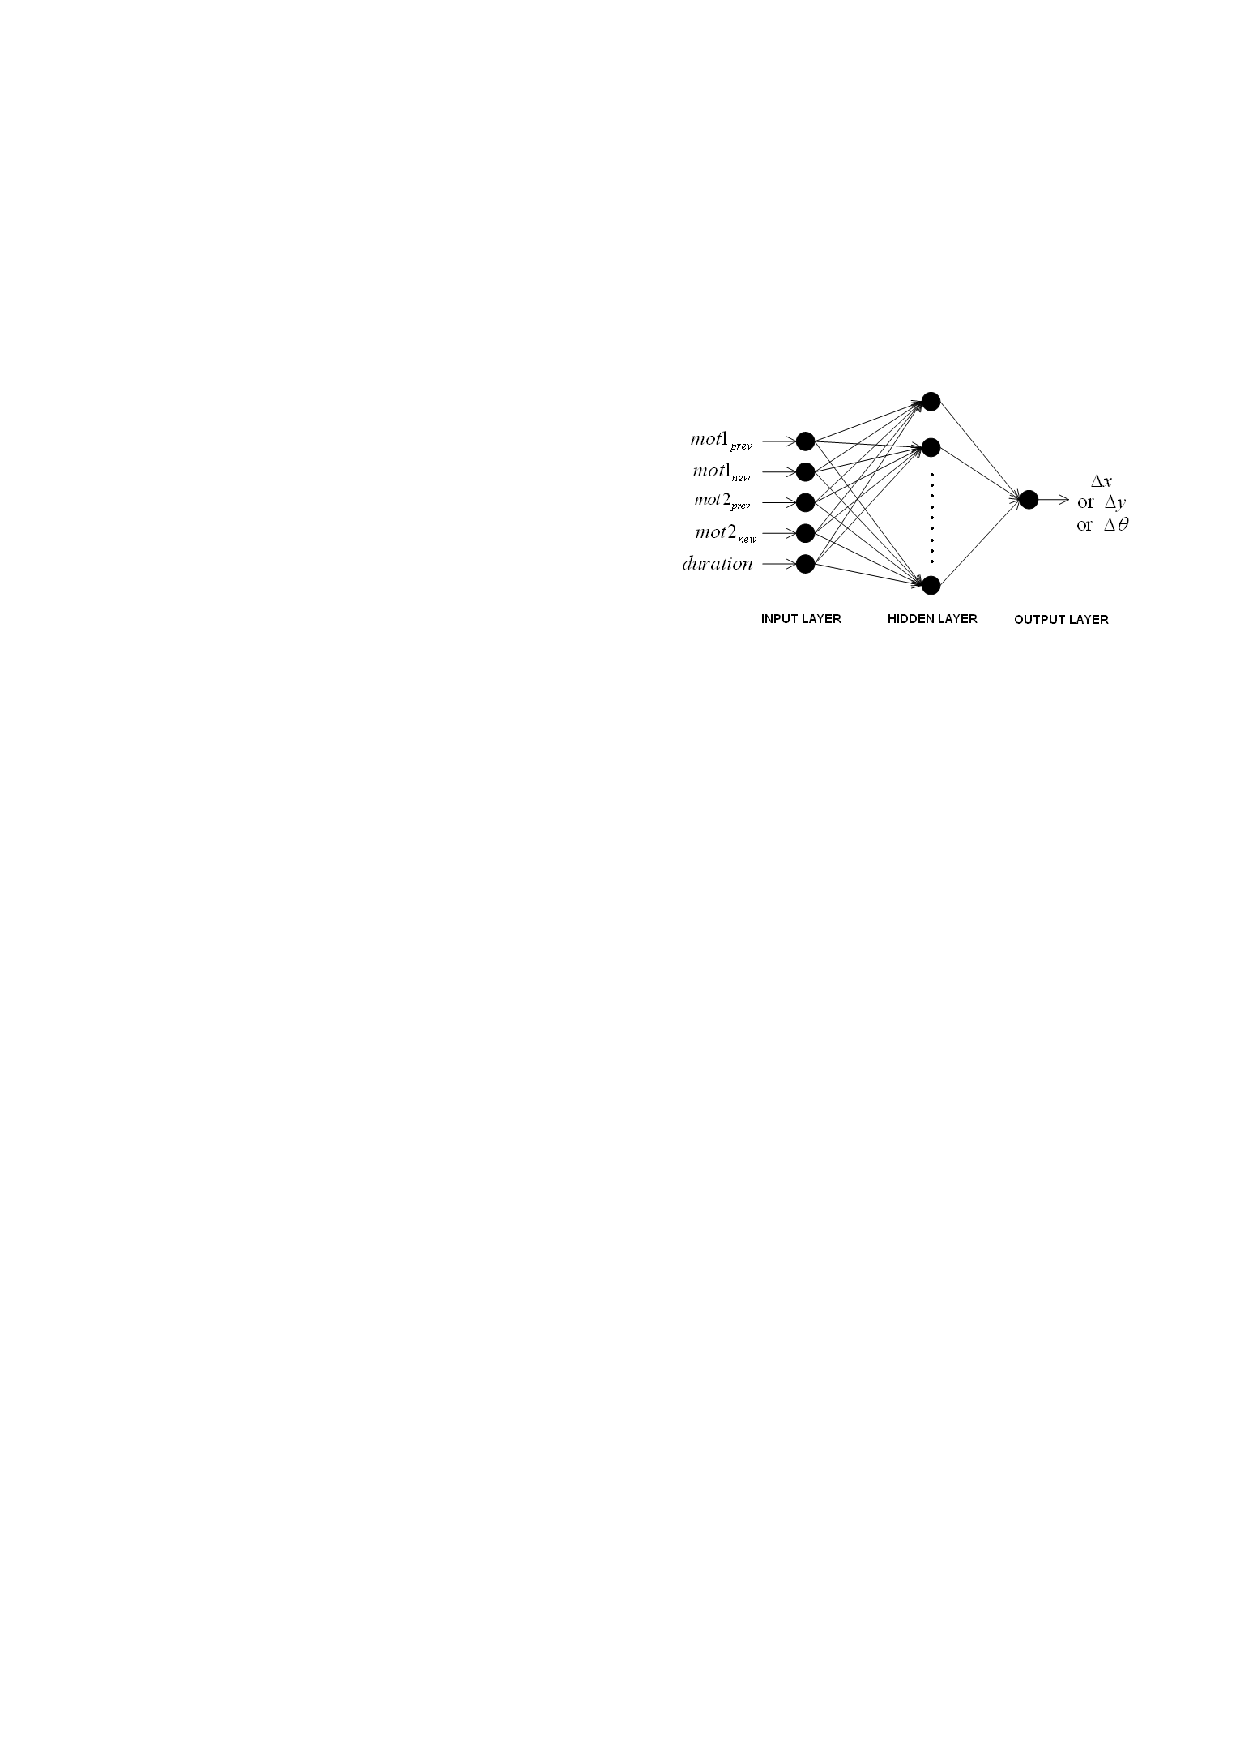
\includegraphics[width=0.95\textwidth]{Illustrations/cr2.pdf}
       \\
     \only{\tiny{ Pretorius $et~al.$}}% \\ \url{http://tr.im/pWUi} }}
\end{column}
\end{columns}
\end{frame}

\section{Research Cases}

\subsection{Station Keeping Robot}
\begin{frame}
  \frametitle{Station Keeping Robot}
\begin{center}
 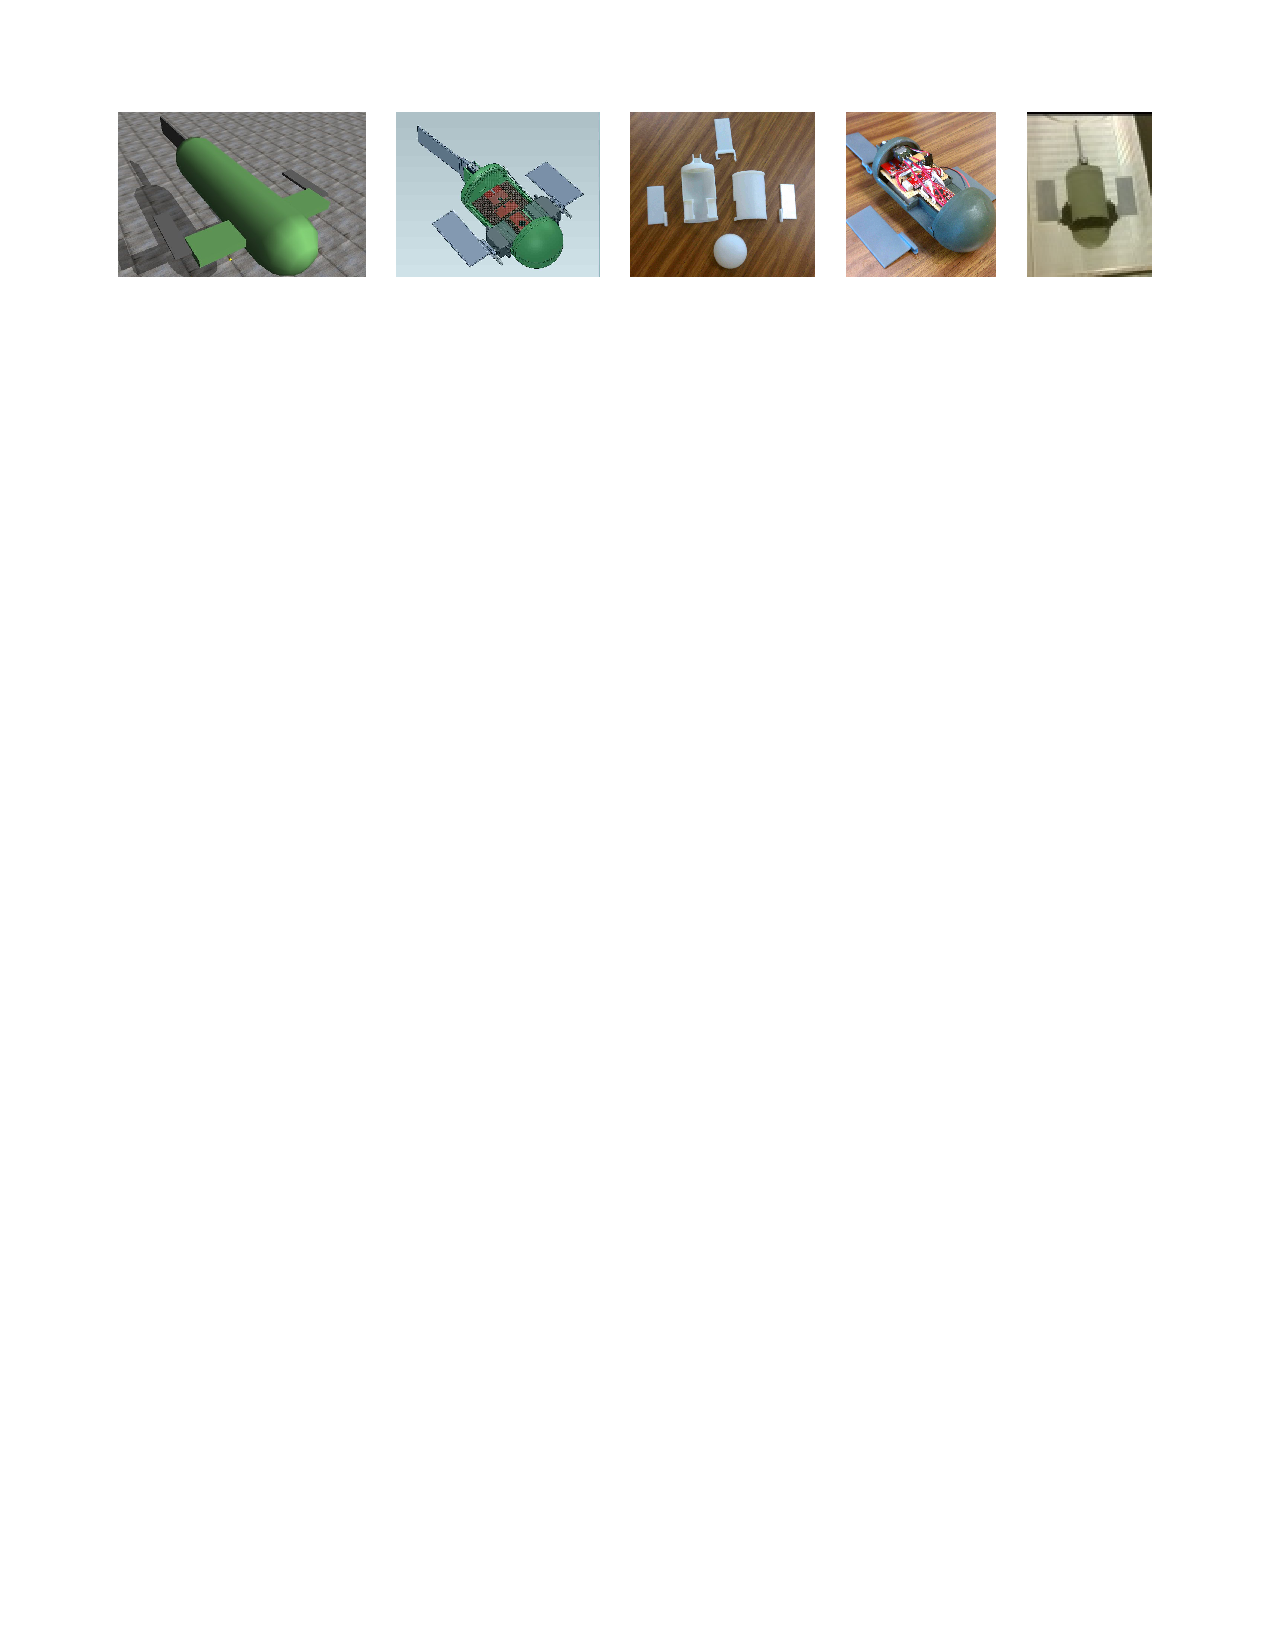
\includegraphics[width=0.95\textwidth]{Illustrations/sr2.pdf}
       \\
    \only{\tiny{Moore $et~al.$}}% \\ \url{http://tr.im/pWUi} }}
\end{center}
\begin{itemize}
\item \large Moore $et~al.$ developed the station keeping robot
\item \large Goal: to maintain position in a body of water
\end{itemize}
\end{frame}

\begin{frame}
  \frametitle{Station Keeping Robot}
\begin{center}
 \includegraphics[width=0.57\textwidth]{Illustrations/sr4.pdf}
       \\
    \only{\tiny{Moore $et~al.$}}% \\ \url{http://tr.im/pWUi} }}
\end{center}

\end{frame}

\subsection{Walking Robot}
\begin{frame}
  \frametitle{Walking Robot}

\begin{columns}
  \begin{column}{0.5\textwidth}
\begin{itemize}
\item  Farchy $et~al.$ modified the code of the Aldebaran Nao robot
\item Goal: to increase walking speed
\end{itemize}
\end{column}
\begin{column}{0.5\textwidth}
 \includegraphics[width=0.95\textwidth]{Illustrations/wr1.pdf}
       \\
    \only{\tiny{Farchy $et~al.$}}% \\ \url{http://tr.im/pWUi} }}
\end{column}
\end{columns}
\end{frame}

\subsection{Coordinate Tracking Robot}
\begin{frame}
  \frametitle{Coordinate Tracking Robot}
\begin{columns}
  \begin{column}{0.5\textwidth}
\begin{itemize}
\item  Pretorius $et~al.$ created a Lego Mindstorms robot
\item Goal: to evolve an internal navigation controller
\end{itemize}
\end{column}
\begin{column}{0.5\textwidth}
 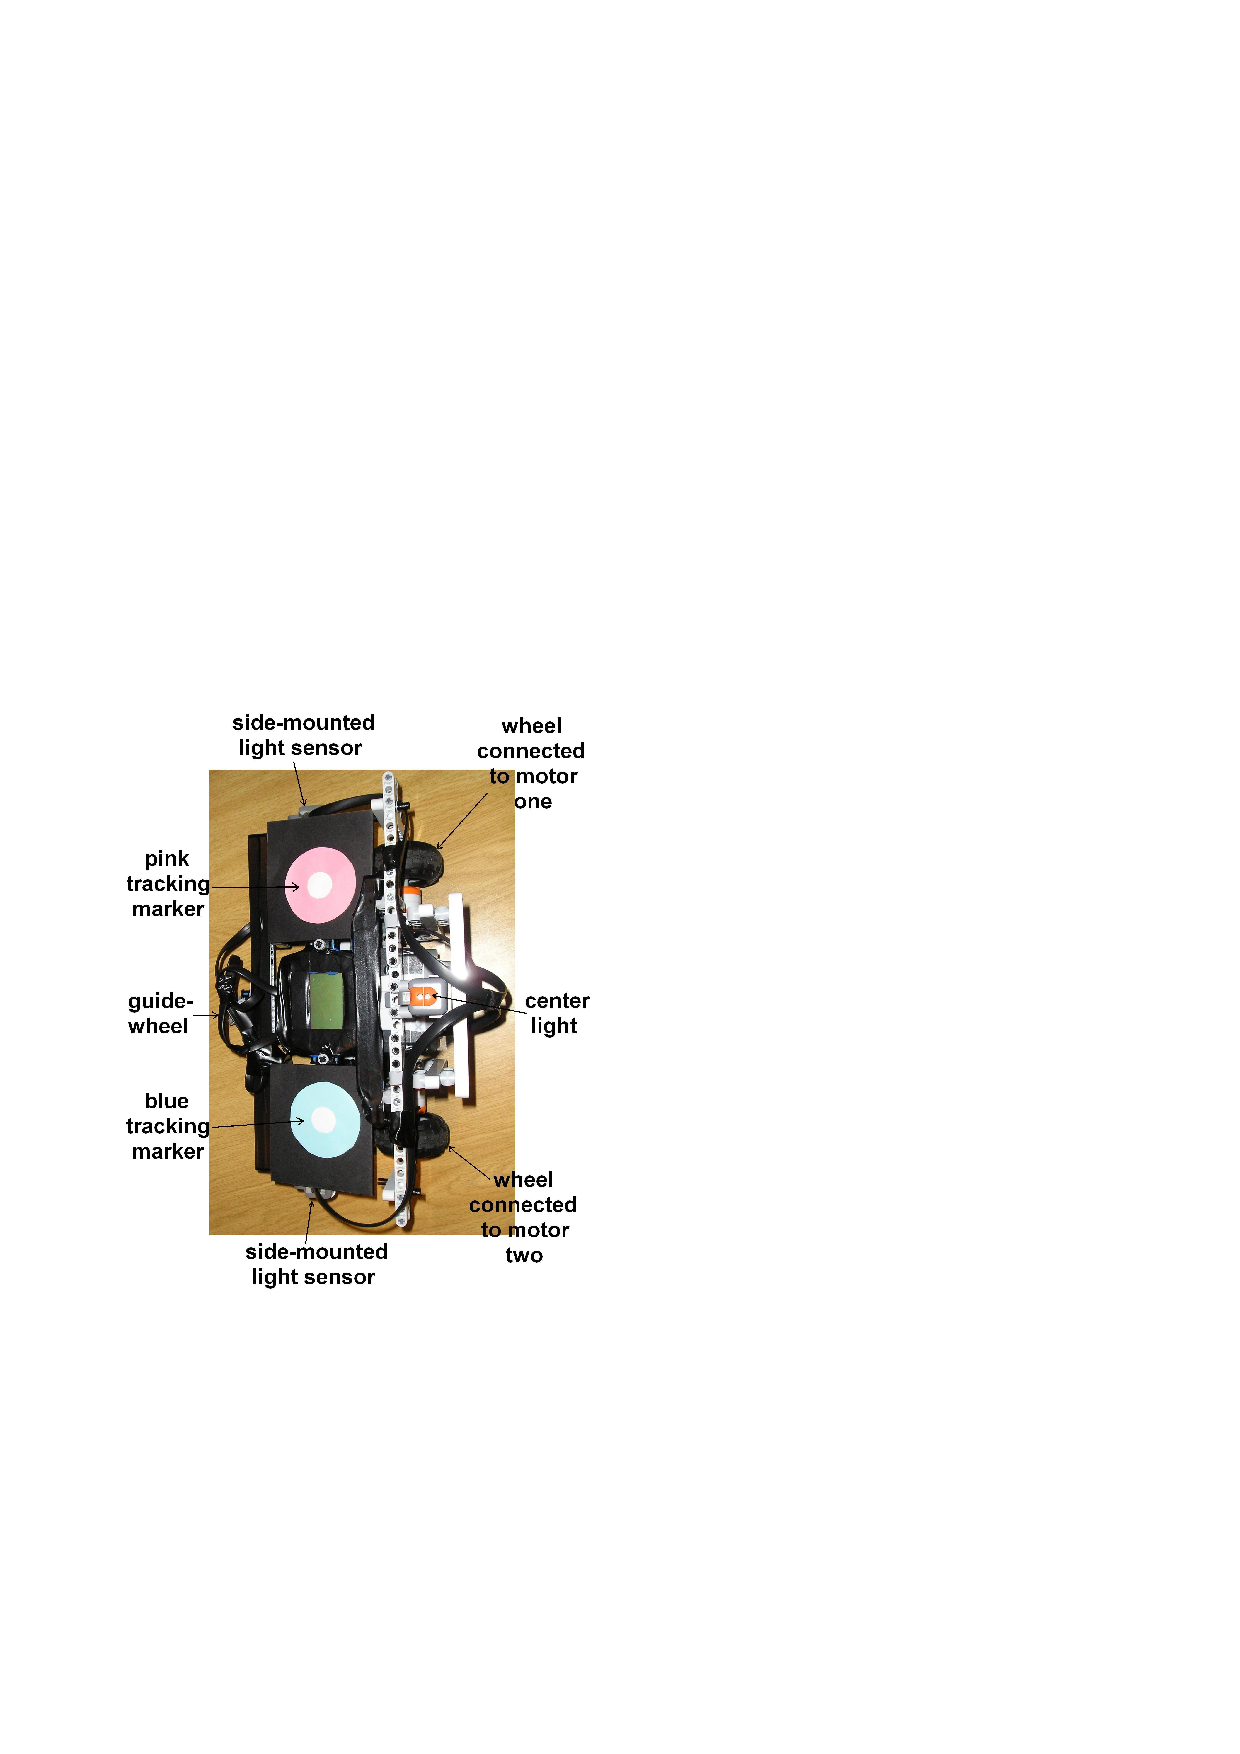
\includegraphics[width=0.95\textwidth]{Illustrations/cr1.pdf}
       \\
    \only{\tiny{ Pretorius $et~al.$}}% \\ \url{http://tr.im/pWUi} }}
\end{column}
\end{columns}
\end{frame}

\section{Simulation}

\subsection{}
\begin{frame}
\frametitle{Simulation}
\begin{itemize}
\item Defined as representing the characteristics or behaviors of one system through the use of another
\item Error caused from inaccuracies of simulation is known as Transitivity 
\end{itemize}
\end{frame}

\subsection{Station Keeping Robot: Simulation}
\begin{frame}
  \frametitle{Station Keeping Robot: Simulation}
\begin{columns}
  \begin{column}{0.5\textwidth}
\begin{itemize}
\item  Used ODE to replicate the robot
\item  No fluid dynamics
\end{itemize}
\end{column}
\begin{column}{0.5\textwidth}
 \includegraphics[width=0.95\textwidth]{Illustrations/sr6.pdf}
       \\
    \only{\tiny{Moore $et~al.$}}% \\ \url{http://tr.im/pWUi} }}
\end{column}
\end{columns}
\end{frame}

\subsection{Walking Robot: Simulation}
\begin{frame}
  \frametitle{Walking Robot: Simulation}
\begin{columns}
  \begin{column}{0.5\textwidth}
\begin{itemize}
\item  Uses SimSpark (also ODE)
\item  Not a perfect representation
\end{itemize}
\end{column}
\begin{column}{0.5\textwidth}
 \includegraphics[width=0.95\textwidth]{Illustrations/wr2.pdf}
       \\
    \only{\tiny{Farchy $et~al.$}}% \\ \url{http://tr.im/pWUi} }}
\end{column}
\end{columns}
\end{frame}

\subsection{Coordinate Tracking Robot: Simulation}
\begin{frame}
  \frametitle{Coordinate Tracking Robot: Simulation}
\begin{itemize}
\item An overhead camera captured heading/orientation of robot from arbitrary motor commands
\item A testbed of 5000 commands were sent to the robot and captured by the camera, creating map of command and position
\end{itemize}
\end{frame}

\section{Evolutionary Process}

\subsection{Station Keeping Robot: Evolutionary Process}
\begin{frame}
  \frametitle{Station Keeping Robot}
\begin{itemize}
\item Evolved a separate candidate for each of the trials
\item Population size of 100 candidates
\item Evolved for 2000 generations
\item The entire process was repeated 25 times for each of the four trials
\end{itemize}
\end{frame}

\begin{frame}
  \frametitle{Station Keeping Robot: Neural Network}
\begin{itemize}
\item Input: 
\begin{itemize}
\item Current 3D coordinates, $(x,y,z)$
\item The difference between current and desired coordinate  $(x,y,z)$
\item The output of the previous output (servo speeds and oscillations)
\end{itemize}
\item Output:
\begin{itemize}
\item oscillation of the rear fin
\item speed of the left flipper
\item speed of the right flipper
\end{itemize}
\end{itemize}
%Neural Network (45 sec)
%Fitness function (45 sec)
%Tweaks to fitness function (1 min)
\end{frame}

\begin{frame}
  \frametitle{Station Keeping Robot: Fitness Function}
\begin{equation*}
	\textrm{fitness} = \sum_{t} (10 - d_t(x, y, z))
\end{equation*}
~~~~~~~~~~~  where
\[
	d_t(x, y, z) = 
		\begin{cases} 10, & \textrm{if distance}_t(x, y, z) > 10 \\
					  \textrm{distance}_t(x, y, z), & \textrm{ otherwise}
		\end{cases}
\]
\begin{itemize}
\item After a 60 second setup phase, fitness was evaluated every 250ms for 60 seconds
\end{itemize}
\end{frame}

%\begin{frame}
  %\frametitle{Station Keeping Robot: Fitness Function}
%\begin{itemize}
%\item After a 60 second setup phase, fitness was evaluated every 250ms for 60 seconds
%\end{itemize}
%\end{frame}

%\subsection{Walking Robot: Evolutionary Process}
%\begin{frame}
%  \frametitle{Walking Robot}
%\begin{itemize}
%\item Farchy $et~al.$ wanted to optimize several parameters to increase speed
%\end{itemize}
%\end{frame}

\subsection{Walking Robot: Evolutionary Process}
\begin{frame}
  \frametitle{Walking Robot: Parameter optimization}
\begin{itemize}
\item Farchy $et~al.$ wanted to optimize several parameters to increase speed
\end{itemize}
\begin{center}
 \includegraphics[scale=1]{Illustrations/wr5.pdf}
       \\
    \only{\tiny{Farchy $et~al.$}}% \\ \url{http://tr.im/pWUi} }}
\end{center}
%Fitness function (1 min)
%GSL (2 min)
\end{frame}

\begin{frame}[fragile]
  \frametitle{Walking Robot: Fitness Functions}
\begin{itemize}
\item Used two fitness functions for two separate runs
\begin{itemize}
\item $omniWalk$
\[
  \textrm{fitness}\_g = (\sum_{t} (\textrm{DistanceTraveled}_t)) - \textrm{fallingPenalty}
\]
\item $WalkFront$
\[
  \textrm{fitness}\_w = \textrm{ maxVelocity() in 15 seconds} \qquad\qquad\quad
\]
\end{itemize}
\end{itemize}

%Fitness function (1 min)
%GSL (2 min)
\end{frame}

\begin{frame}
  \frametitle{Walking Robot: Grounded Simulation Learning}
  \begin{itemize}
  \item Farchy $et~al.$ used Grounded Simulation Learning (GSL) when evolving candidates
  \item The point of GSL is to add human guidance in the evolution process
  \item This is done by examining the physical robot with an evolved candidate implementation, and isolating particular attributes
  \end{itemize}
\end{frame}

\subsection{Coordinate Tracking Robot: Evolutionary Process}
\begin{frame}
  \frametitle{Coordinate Tracking Robot}
  \begin{itemize}
   \item Population of 250 candidates
   \item Evolved for 15,000 generations
   \item Process repeated three times for each ANN

  \end{itemize}
%Explain commands (45 sec)
%Neural Network (45 sec)
%Fitness function (1 min)
%Explain nav controller (1:30 min)
\end{frame}



\begin{frame}
  \frametitle{Coordinate Tracking Robot: Artificial Neural Network}
  \begin{columns}
  \begin{column}{0.5\textwidth}
\begin{itemize}
\item Navigational controller consists of three ANN:
\begin{itemize}
\item The x-coordinate,
\item The y-coordinate,
\item And the angle
\end{itemize}
\item Inputs of the ANNs:
\begin{itemize}
\item Current Motor speeds
\item Current length of time
\item Previous Motor speeds
\end{itemize}
\end{itemize}
\end{column}
\begin{column}{0.5\textwidth}
 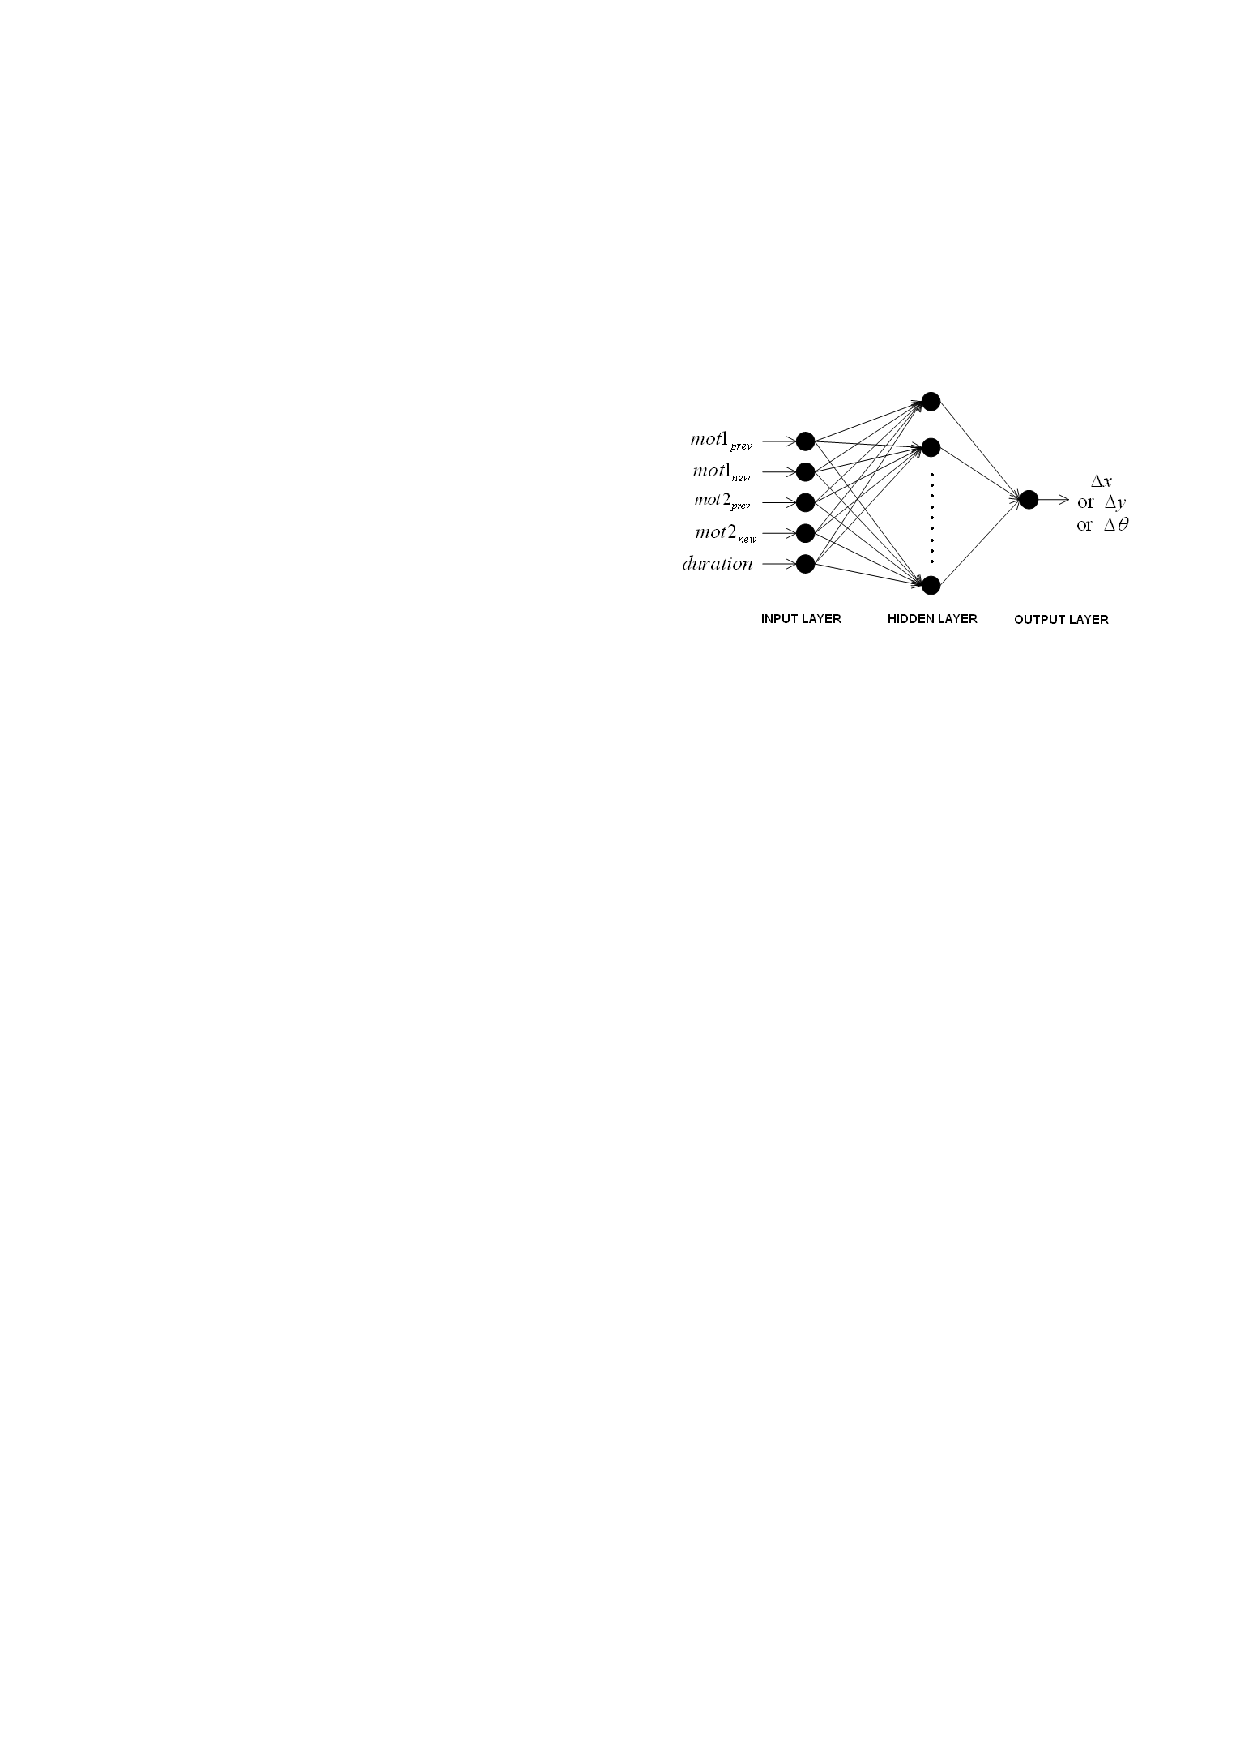
\includegraphics[width=0.95\textwidth]{Illustrations/cr2.pdf}
       \\
    \only{\tiny{ Pretorius $et~al.$}}% \\ \url{http://tr.im/pWUi} }}
\end{column}
\end{columns}
%Explain commands (45 sec)
%Neural Network (45 sec)
%Fitness function (1 min)
%Explain nav controller (1:30 min)
\end{frame}

\begin{frame}[fragile]
\frametitle{Coordinate Tracking Robot: Fitness Function}
\begin{itemize}
\item Used the Mean Squared Error (MSE) as the fitness function
\end{itemize}
  \[
  \textrm{fitness} = \frac{1}{N}\sum\limits_{p=1}^N\sum\limits_{i=1}^O (t_{pi} - a_{pi})^2,
\] 

%\begin{itemize}
%\item N is the size of the testbed (5,000) %more?
%\end{itemize}
\end{frame}

%\begin{frame}
%\frametitle{Coordinate Tracking Robot: Commands}
%\begin{itemize}
%\item A command is a data structure used by Pretorius $et~al.$ is 
%\item Commands encapsulate:
%\begin{itemize}
%\item Motor speeds,
%\item Motor directions,
%\item Time of execution
%\end{itemize}
%\end{itemize}
%\end{frame}


\section{Results}
\subsection{Station Keeping Robot: Results} %http://y2u.be/UufbnEGFwV4
\begin{frame}
  \frametitle{Station Keeping Robot: Results}
  \begin{center}
  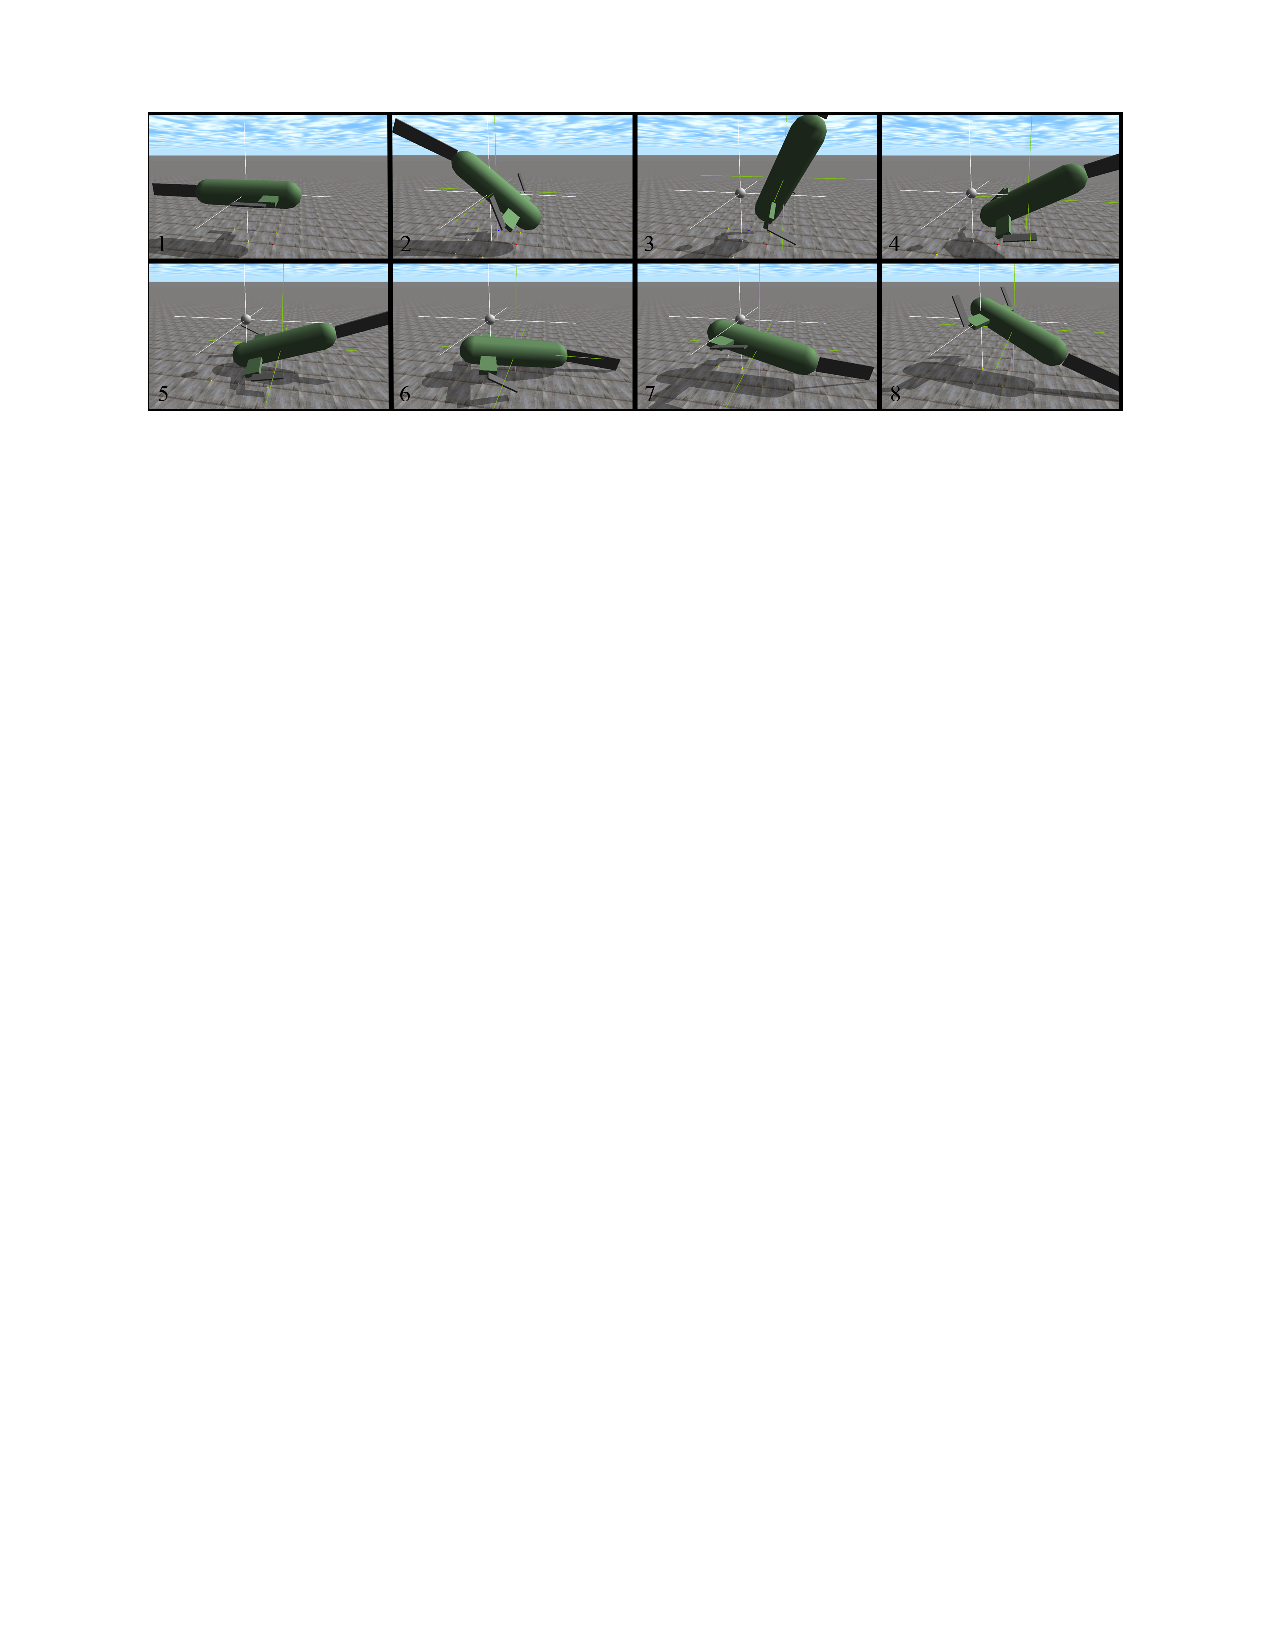
\includegraphics[width=0.75\textwidth]{Illustrations/sr1.pdf}
       \\
    \only{\tiny{Moore et al. }}
    \end{center}
  \begin{itemize}
    \item Each trial had a candidate which successfully maintained the position
        \item When the flow was coming from behind, the evolved candidate would flip end-over-head to orient itself (http://y2u.be/UufbnEGFwV4)
  \end{itemize}
\end{frame}

\begin{frame}
  \frametitle{Walking Robot: Results}

\begin{center}
 \includegraphics[width=0.7\textwidth]{Illustrations/wr4.pdf}
       \\
   \only{\tiny{Farchy $et~al.$}}% \\ \url{http://tr.im/pWUi} }}
\end{center}
\end{frame}

\subsection{ResultsCoordRobot}
\begin{frame}
  \frametitle{Coordinate Tracking Robot: Results}
 \begin{itemize}
 \item Each of the ANNs evolved for 12 hours
 \item Pretorius $et~al.$ noted that the results were reasonably accurate
\begin{center}
 \includegraphics[scale=1.25]{Illustrations/cr4.pdf}
       \\
    \only{\tiny{ Pretorius $et~al.$}}% \\ \url{http://tr.im/pWUi} }}
\end{center}
\end{itemize}
\end{frame}

\begin{frame}
\frametitle{Coordinate Tracking Robot: Navigation Test}
\begin{itemize}
\item Using the evolved ANNs, a navigation test was made for a practical application
\item The test was evolved to:
\begin{itemize}
\item Drive the robot in a circle around a 3x3 grid,
\item Not leave the grid or touch the middle square
\end{itemize}
\end{itemize}
\end{frame}

\begin{frame}
  \frametitle{Coordinate Tracking Robot: Results}
\begin{center}
 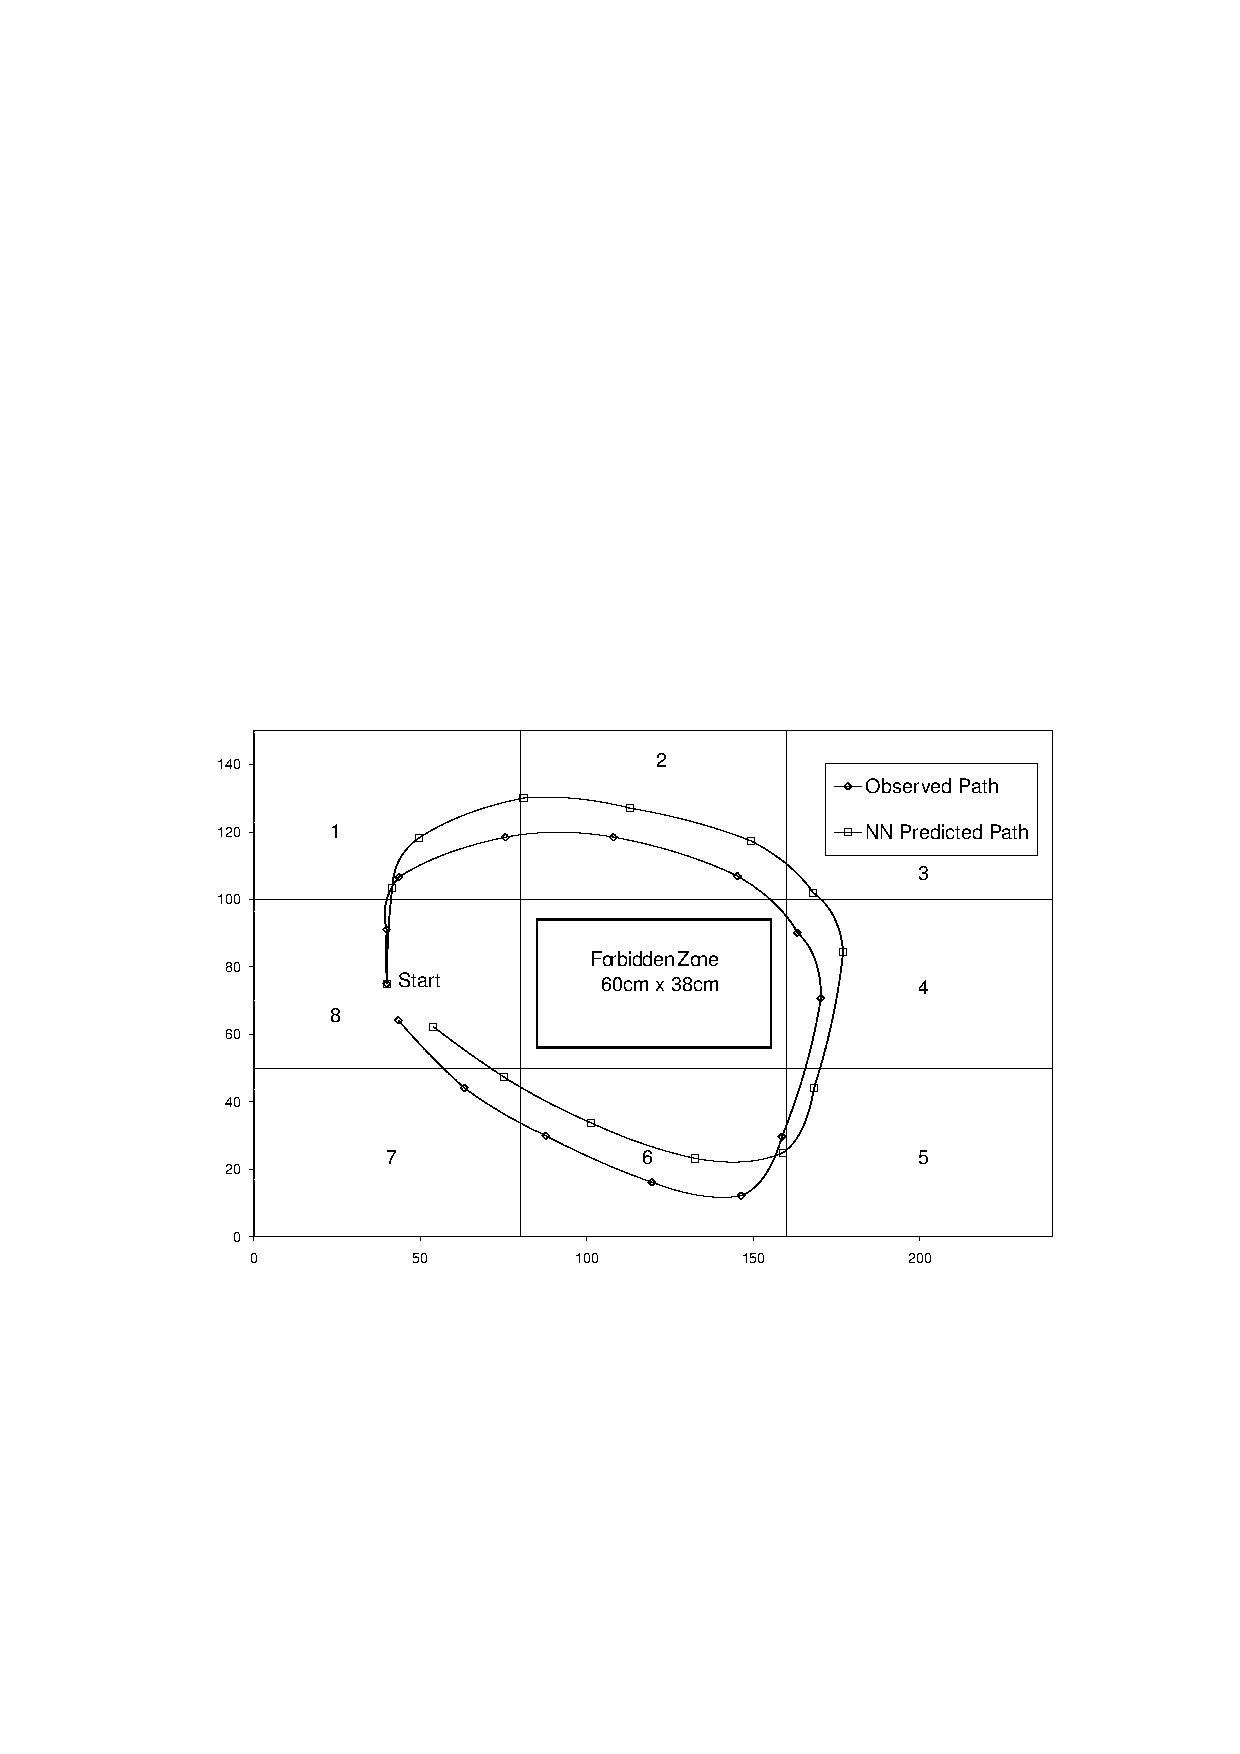
\includegraphics[width=0.7\textwidth]{Illustrations/cr3.pdf}
       \\
    \only{\tiny{ Pretorius $et~al.$}}% \\ \url{http://tr.im/pWUi} }}
\end{center}
\end{frame}

\section{Conclusion}
\subsection{}
\begin{frame}
  \frametitle{Conclusion}
  \begin{itemize}
\item By using a simulation, the evolutionary process can occur at a significantly faster rate
\item Evolutionary robotics could be applied if:
 \begin{itemize}
\item the robotics problem is well defined, %solution is not apparent?
\item the robot and environment can be simulated,
\item and the simulated robot's success can be quantified
\end{itemize}
\end{itemize}
\end{frame}

\section*{Questions and Acknowledgments}
\subsection*{}
\begin{frame}
  \frametitle{}
\begin{center}
Thank you to Nic McPhee, Elena Machkasova, and Alex Jarvis\\
  \large Any Questions? 
\end{center}

\end{frame}

\section*{Resources}
\subsection*{}
\begin{frame}
  \frametitle{}
\begin{center}
  \large asdghdsa 
\end{center}
\end{frame}

\end{document}
